%!TEX root = ./paper.tex
%\section*{Appendix}

\begin{figure}[h]
  \centering 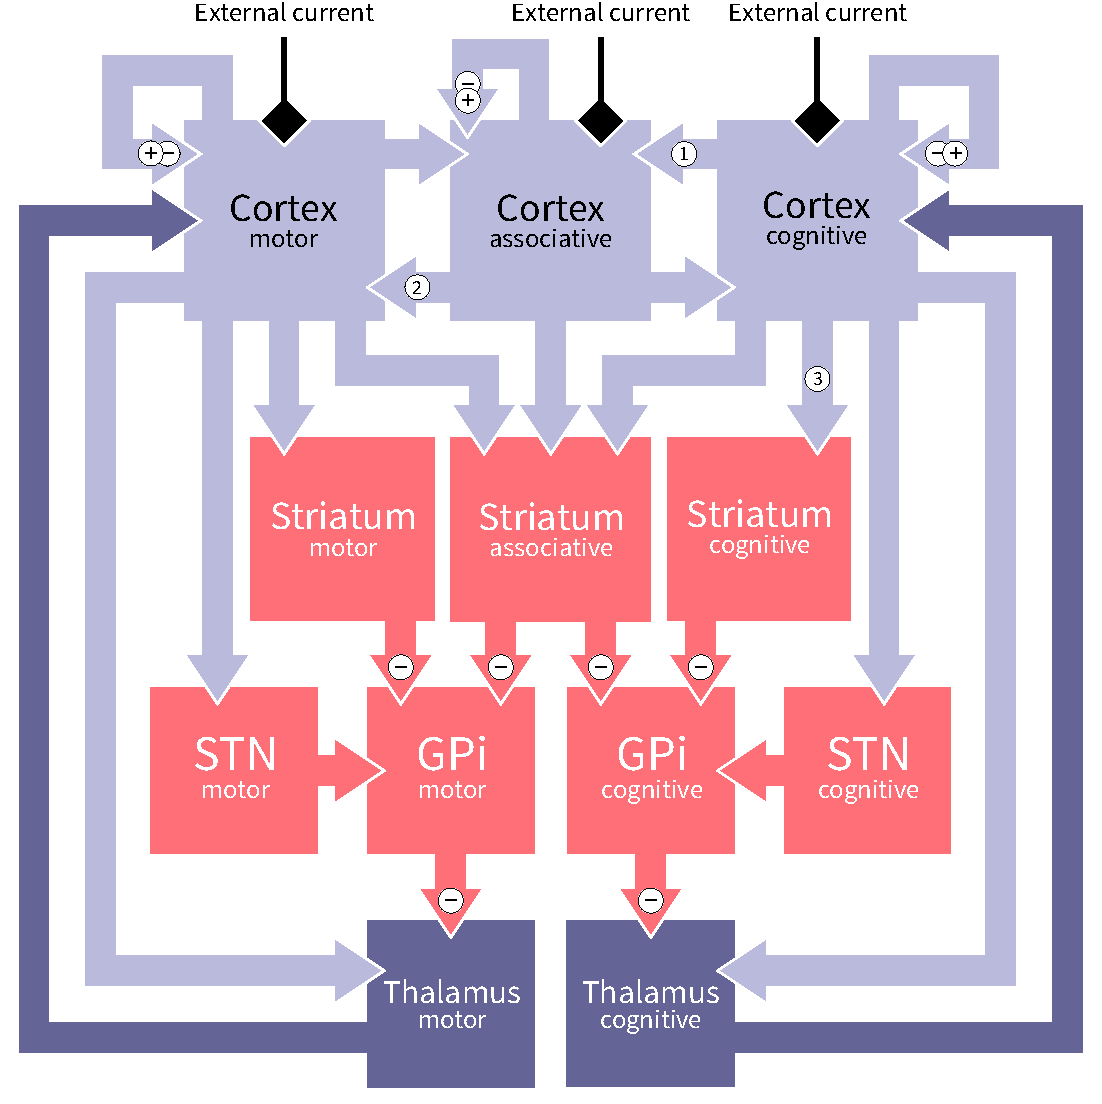
\includegraphics[width=0.75\textwidth]{architecture}
  \caption{The main pathways in the model are the direct pathway
    (Cortex-Striatum-GPi-Thalamus-Cortex) and the hyperdirect pathway
    (Cortex-Striatum-GPi-Thalamus-Cortex). Learning occurs at two different
    levels: Hebbian learning from cognitive to associative cotex (1) and
    reinforcement from cognitive cortex to cognitiv striatum (3).}
  \label{fig:architecture}
\end{figure}



\begin{figure}[h]
        \centering
        \begin{subfigure}[b]{0.4\textwidth}
                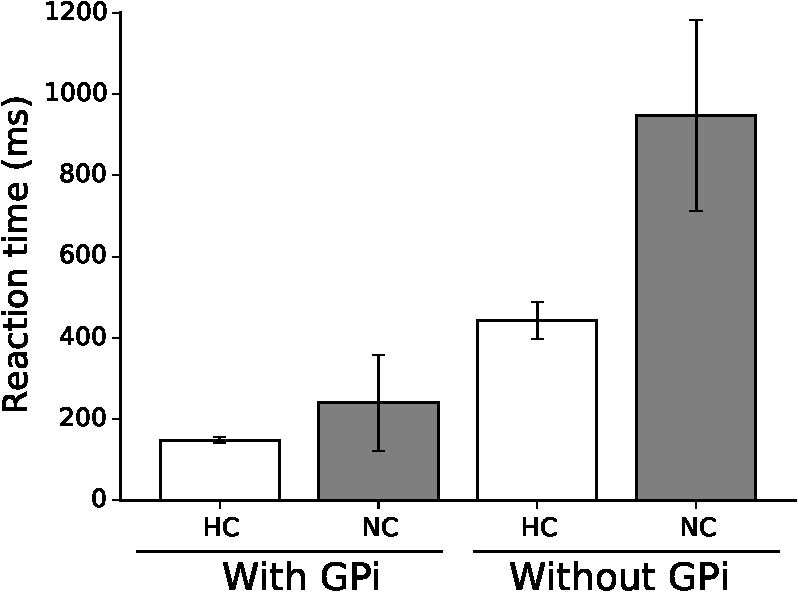
\includegraphics[width=\textwidth]{RTresults}

        		  \vspace{2mm}
                \caption{Mean reaction time}
                \label{fig:RTresults}
        \end{subfigure}
        \vspace{4mm}

        \begin{subfigure}[b]{0.9\textwidth}
                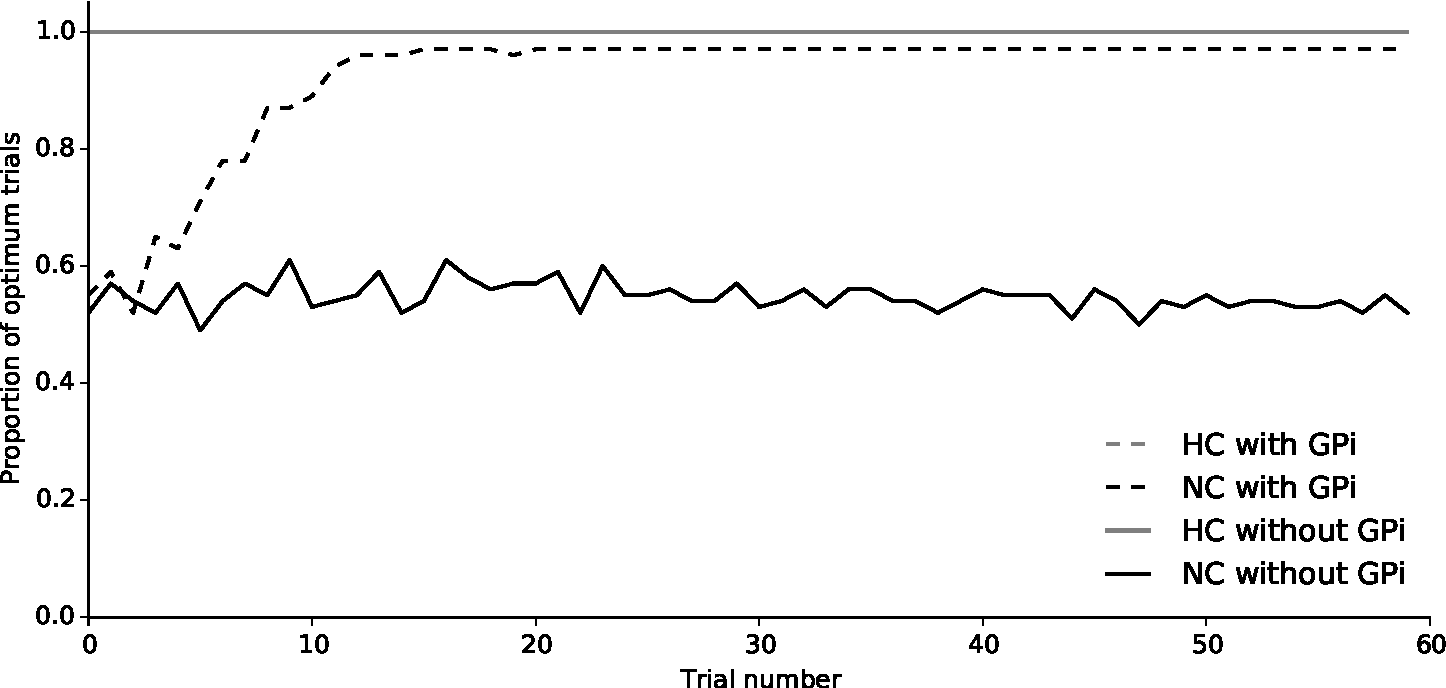
\includegraphics[width=\textwidth]{Performances}
        		  \vspace{2mm}
                \caption{Mean performances}
                \label{fig:Performances}
        \end{subfigure}
        \vspace{4mm}
        \caption{Results. \ref{fig:RTresults}) Analysis of the data shows that
          reaction time is higher in NC as compared to HC with active and
          inactive GPi. The later increases significantly the reaction time in
          both conditions.  \ref{fig:Performances}) In HC, performances are
          optimal (1), with or wthout GPi. In NC, only the intact model (with
          GPi) is able to learn the new stimuli while lesioned model
          performances stay at the level f chance.}
\end{figure}
